\documentclass{ximera}

\graphicspath{{./content/02_6_curvature/graphics/}{./graphics/}}

\title{Curvature}
\author{Melissa Lynn}
\outcome{Understand the definition and geometric significance of curvature. Compute curvature. Understand the definition of the osculating circle.}

\begin{document}
\begin{abstract}
\end{abstract}
\maketitle

We have an intuitive idea for what it means for a curve to be ``curvy.'' Intuitively, we would probably describe the following curves as ``not very curvy.''

\begin{image}
\begin{tikzpicture}
\draw  (0,0) to[out=55,in=215] (2,2);
\draw  (3,2) to[out=-55,in=125] (5,0);
\draw  (6,1) -- (8,1);
\end{tikzpicture}
\end{image}

On the other hand, we'd probably describe the next group of curves as ``very curvy.''

\begin{image}
\begin{tikzpicture}
\draw  (0,0) to[out=175,in=185] (0,2);
\draw  (0,2) to[out=5,in=-5] (2,0);
\draw  (2,0) to[out =175,in=175] (1,1);

\draw  (4,0) to[out=90,in=180] (4.5,2);
\draw  (4.5,2) to[out=0,in=90] (5,1);
\draw  (5,1) to[out=270,in=180] (5.5,0);
\draw  (5.5,0) to[out=0,in=180] (6,2);
\draw  (6,2) to[out=0,in=180] (8,0);
\end{tikzpicture}
\end{image}

However, we don't yet have a way to represent ``curviness'' mathematically. In this section, we'll define the \emph{curvature} of a curve, which will allow us to quantify ``curviness.'' 

In order to ensure that our definition is independent of the parametrization, we'll need to work with the arclength parametrization $\vec{x}(s)$. Recall that this parametrization traverses the curve at unit speed.

\section*{Definition of Curvature}

Let's look at the behavior of the unit tangent vector as we traverse various curves. The unit tangent vector is the velocity divided by the speed, so
\[
\vec{T}(t) = \frac{\vec{x}'(t)}{\|\vec{x}'(t)\|}.
\]
Since the arclength parametrization has unit speed, we have
\[
\vec{T}(s) = \vec{x}'(s).
\]

\youtube{h6NFSX12Zpw}

We see that the unit tangent vector changes very quickly when we're curving sharply, and the unit tangent vector doesn't change when we're going straight. So, we'll use the change in the unit tangent vector to measure ``curviness.''

\begin{definition}
Suppose the arclength parametrization of a curve $C$ is $\vec{x}(s)$. Then we define the \emph{curvature} of $C$ at time $s$ to be
\[
\kappa(s) = \|\vec{T}'(s)\|.
\]
\end{definition}

Unfortunately, as we've seen, it's not always easy to find an arclength parametrization for a curve. Fortunately, we can still compute the curvature without finding an arclength parametrization.

Suppose we have a parametrization $\vec{x}(t)$ of a curve. Then, thinking of $s$ as a function of $t$ and using the chain rule,
\[
\vec{T}'(t) = \vec{T}'(s)s'(t).
\]
Then $\vec{T}'(s) = \frac{\vec{T}'(t)}{s'(t)}$. Recalling that $s'(t)$ is the speed of the parametrization $\vec{x}(t)$, we can compute the curvature as follows.

\begin{proposition}
Let $\vec{x}(t)$ be a parametrization of a curve $C$. Then
\[
\kappa(t) = \frac{\|\vec{T}'(t)\|}{\|\vec{x}'(t)\|}.
\]
\end{proposition}

We'll typically use this equation to compute curvature.

\section*{Computing Curvature}

\begin{example}
We'll compute the curvature of a circle of radius $a>0$, parametrized by $\vec{x}(t) = (a\cos(t), a\sin(t))$.

In order to find the unit tangent vector, we'll need to compute the velocity and speed.
\[
\vec{x}'(t) = \answer{(-a\sin(t), a\cos(t))}
\]
Then the speed of $x(t)$ is
\[
\|\vec{x}'(t)\| = \answer{a}.
\]
Dividing the velocity by the speed, we obtain the unit tangent vector,
\[
\vec{T}(t) = \answer{(-\sin(t),\cos(t))}.
\]
Now, we find $\vec{T}'(t)$.
\[
\vec{T}'(t) = (-cos(t),-sin(t))
\]
The magnitude of this vector is $\answer{1}$.

Finally, we compute the curvature at time $t$.
\[
\kappa(t) = \frac{\|\vec{T}'(t)\|}{\|\vec{x}'(t)\|} = \answer{\frac{1}{a}}
\]
Note that the curvature is independent of the time $t$, so independent of our position on the circle. This matches with the symmetry of the circle.

\begin{image}
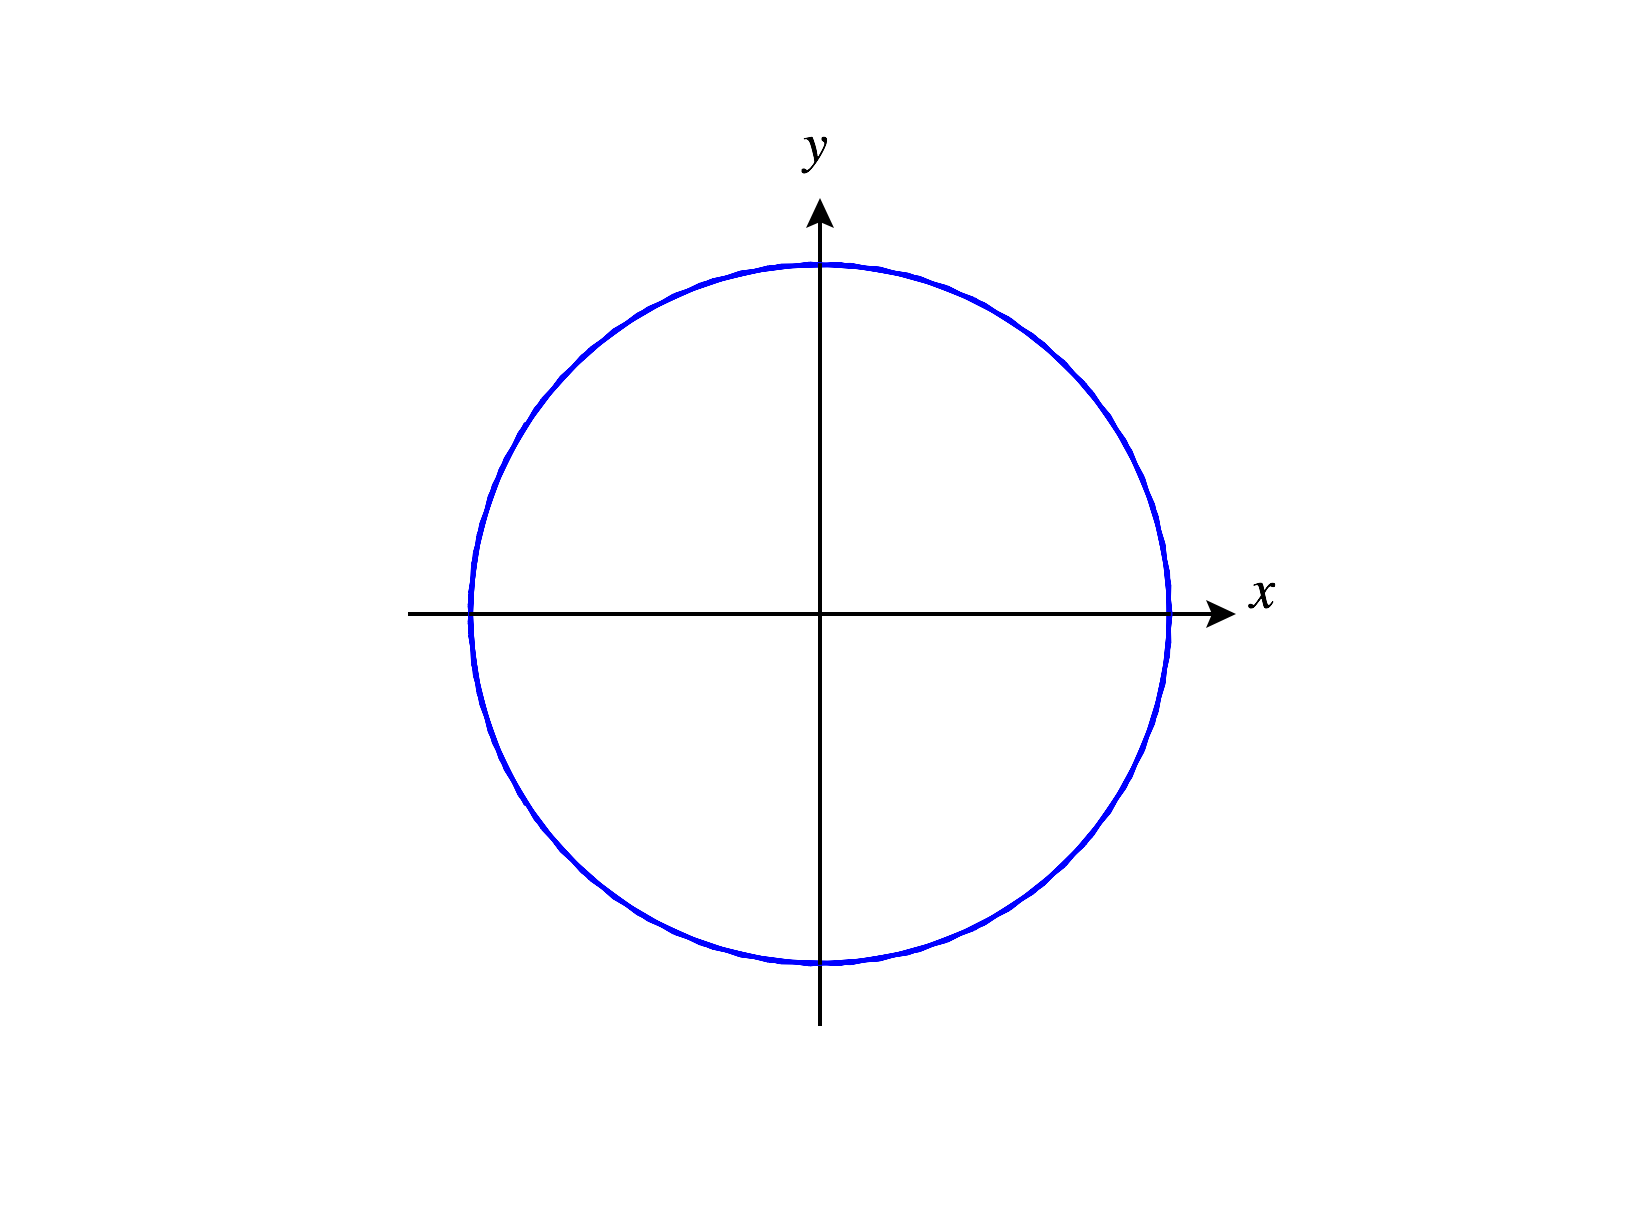
\includegraphics[width=\textwidth]{CalcPlot3D-generic_circle}
\end{image}
\end{example}

\begin{example}
We'll compute the curvature of the path $\vec{x}(t) = (t\cos(t),t\sin(t), t^2)$, for $t\geq 0$.

In order to find the unit tangent vector, we'll need to compute the velocity and speed.
\[
\vec{x}'(t) = \answer{(-t\sin(t), t\cos(t),2t)}
\]
Then the speed of $x(t)$ is
\[
\|\vec{x}'(t)\| = \answer{\sqrt{5}t}.
\]
Dividing the velocity by the speed, we obtain the unit tangent vector,
\[
\vec{T}(t) = \answer{(\frac{-1}{\sqrt{5}}\sin(t),\frac{1}{\sqrt{5}}\cos(t), \frac{2}{\sqrt{5}})}.
\]
Now, we find $\vec{T}'(t)$.
\[
\vec{T}'(t) = (\frac{-1}{\sqrt{5}}\cos(t),\frac{-1}{\sqrt{5}}\sin(t), 0)
\]
The magnitude of this vector is $\answer{\sqrt{5}}$.

Finally, we compute the curvature at time $t$.
\[
\kappa(t) = \frac{\|\vec{T}'(t)\|}{\|\vec{x}'(t)\|} = \answer{\frac{1}{t}}
\]
\end{example}

\section*{Osculating Circle}

In a previous example, we found that the curvature of the circle of radius $a$ is constant, and $\kappa = \frac{1}{a}$. Another way to say this is that the radius of the circle is ``one over the curvature,'' or $a = \frac{1}{\kappa}$. We can extend this idea to other curves as well: given $\vec{x}(t)$, $r = \frac{1}{\kappa(t)}$ is the radius of the circle which ``best fits'' the graph at time $t$. We call this circle the \emph{osculating circle} at that point.

In the following video, you can see how the osculating circle changes as we traverse a curve.

\youtube{VkTSpo8e4Mc}


\textit{Images were generated using \href{https://www.monroecc.edu/faculty/paulseeburger/calcnsf/CalcPlot3D/}{CalcPlot3D}.}

\end{document}